\documentclass[tikz,border=8pt]{standalone}
\usepackage[utf8]{inputenc}
\usepackage[T1]{fontenc}
\usepackage{amsmath}
\usepackage{graphicx}
\usetikzlibrary{arrows.meta,positioning,fit,backgrounds,calc,shapes.geometric}

\tikzset{
  >=Latex,
  fixed/.style={draw, rounded corners, fill=blue!8, align=center,
    minimum height=8mm, text width=33mm, font=\scriptsize},
  hyper/.style={draw, rounded corners, fill=violet!10, align=center,
    minimum height=8mm, text width=31mm, font=\scriptsize},
  latent/.style={draw, circle, fill=white, align=center,
    minimum size=10mm, font=\scriptsize},
  latentwide/.style={draw, rounded corners, fill=white, align=center,
    minimum height=8mm, text width=31mm, font=\scriptsize},
  observed/.style={draw, rounded corners, fill=black!12, align=center,
    minimum height=10mm, text width=38mm, font=\scriptsize},
  det/.style={draw, diamond, aspect=2.4, fill=yellow!18, align=center,
    inner sep=1.4pt, text width=43mm, font=\scriptsize},
  output/.style={draw, rounded corners, fill=yellow!15, align=left,
    minimum height=10mm, text width=47mm, font=\scriptsize},
  panel/.style={draw, rounded corners, dashed, inner sep=5mm},
  arr/.style={-{Latex[length=2mm]}, line width=.55pt}
}

\begin{document}
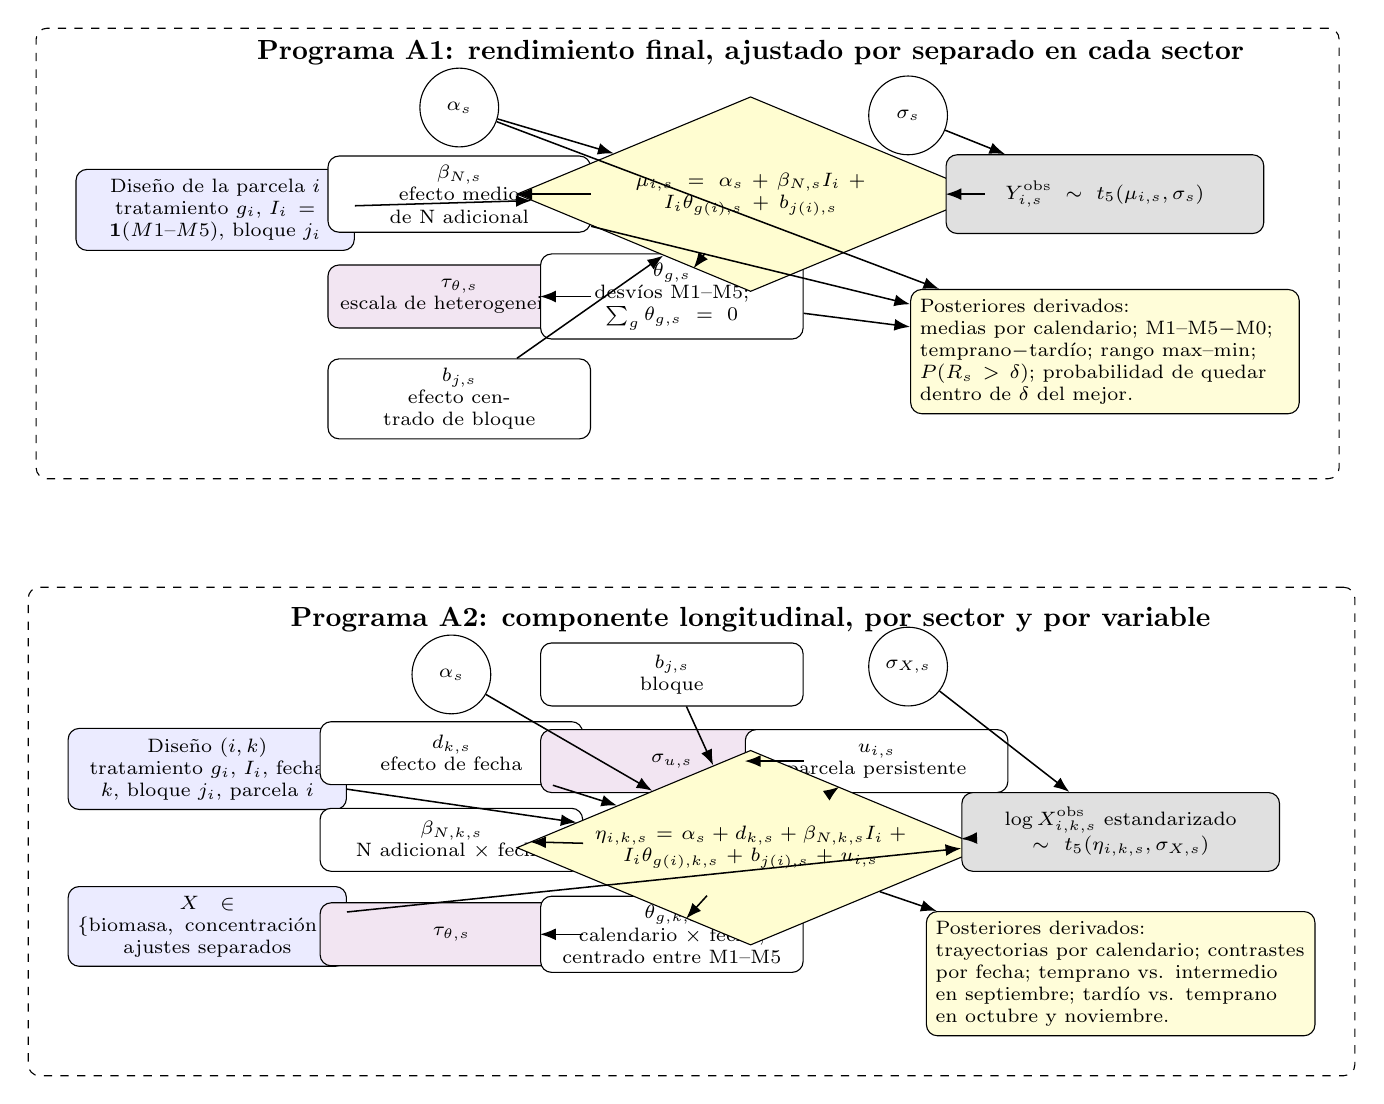
\begin{tikzpicture}[x=1cm,y=1cm]

% ------------------------------------------------------------------
% A1: final yield
% ------------------------------------------------------------------
\node[font=\bfseries] at (7.0,4.7)
  {Programa A1: rendimiento final, ajustado por separado en cada sector};

\node[fixed] (designY) at (0.2,2.7)
  {Diseño de la parcela $i$\\tratamiento $g_i$, $I_i=\mathbf 1(M1\text{--}M5)$, bloque $j_i$};
\node[latent] (alphaY) at (3.3,4.0) {$\alpha_s$};
\node[latentwide] (betaY) at (3.3,2.9) {$\beta_{N,s}$\\efecto medio de N adicional};
\node[hyper] (tauY) at (3.3,1.6) {$\tau_{\theta,s}$\\escala de heterogeneidad};
\node[latentwide] (thetaY) at (6.0,1.6)
  {$\theta_{g,s}$\\desvíos M1--M5; $\sum_g\theta_{g,s}=0$};
\node[latentwide] (blockY) at (3.3,0.3) {$b_{j,s}$\\efecto centrado de bloque};
\node[latent] (sigmaY) at (9.0,3.9) {$\sigma_s$};

\node[det] (muY) at (7.0,2.9)
  {$\mu_{i,s}=\alpha_s+\beta_{N,s}I_i+I_i\theta_{g(i),s}+b_{j(i),s}$};
\node[observed] (obsY) at (11.5,2.9)
  {$Y_{i,s}^{\mathrm{obs}}\sim t_5(\mu_{i,s},\sigma_s)$};
\node[output] (outY) at (11.5,0.9)
  {Posteriores derivados:\\
   medias por calendario; M1--M5$-$M0; temprano$-$tardío; rango max--min; $P(R_s>\delta)$; probabilidad de quedar dentro de $\delta$ del mejor.};

\draw[arr] (tauY) -- (thetaY);
\draw[arr] (designY) -- (muY);
\draw[arr] (alphaY) -- (muY);
\draw[arr] (betaY) -- (muY);
\draw[arr] (thetaY) -- (muY);
\draw[arr] (blockY) -- (muY);
\draw[arr] (muY) -- (obsY);
\draw[arr] (sigmaY) -- (obsY);
\draw[arr] (alphaY) -- (outY);
\draw[arr] (betaY) -- (outY);
\draw[arr] (thetaY) -- (outY);

\begin{scope}[on background layer]
  \node[panel, fit=(designY)(alphaY)(betaY)(tauY)(thetaY)(blockY)(sigmaY)(muY)(obsY)(outY)] {};
\end{scope}

% ------------------------------------------------------------------
% A2: longitudinal
% ------------------------------------------------------------------
\begin{scope}[yshift=-7.2cm]
\node[font=\bfseries] at (7.0,4.7)
  {Programa A2: componente longitudinal, por sector y por variable};

\node[fixed] (designL) at (0.1,2.8)
  {Diseño $(i,k)$\\tratamiento $g_i$, $I_i$, fecha $k$, bloque $j_i$, parcela $i$};
\node[fixed] (whichL) at (0.1,0.8)
  {$X\in\{\text{biomasa},\ \text{concentración de N}\}$\\ajustes separados};

\node[latent] (alphaL) at (3.2,4.0) {$\alpha_s$};
\node[latentwide] (dateL) at (3.2,3.0) {$d_{k,s}$\\efecto de fecha};
\node[latentwide] (betaL) at (3.2,1.9) {$\beta_{N,k,s}$\\N adicional $\times$ fecha};
\node[hyper] (tauL) at (3.2,0.7) {$\tau_{\theta,s}$};
\node[latentwide] (thetaL) at (6.0,0.7)
  {$\theta_{g,k,s}$\\calendario $\times$ fecha; centrado entre M1--M5};
\node[latentwide] (blockL) at (6.0,4.0) {$b_{j,s}$\\bloque};
\node[hyper] (plotSdL) at (6.0,2.9) {$\sigma_{u,s}$};
\node[latentwide] (plotL) at (8.6,2.9) {$u_{i,s}$\\parcela persistente};
\node[latent] (sigmaL) at (9.0,4.1) {$\sigma_{X,s}$};

\node[det] (etaL) at (7.0,1.8)
  {$\eta_{i,k,s}=\alpha_s+d_{k,s}+\beta_{N,k,s}I_i+I_i\theta_{g(i),k,s}+b_{j(i),s}+u_{i,s}$};
\node[observed] (obsL) at (11.7,2.0)
  {$\log X_{i,k,s}^{\mathrm{obs}}$ estandarizado\\$\sim t_5(\eta_{i,k,s},\sigma_{X,s})$};
\node[output] (outL) at (11.7,0.2)
  {Posteriores derivados:\\trayectorias por calendario; contrastes por fecha; temprano vs. intermedio en septiembre; tardío vs. temprano en octubre y noviembre.};

\draw[arr] (tauL) -- (thetaL);
\draw[arr] (plotSdL) -- (plotL);
\draw[arr] (designL) -- (etaL);
\draw[arr] (whichL) -- (obsL);
\draw[arr] (alphaL) -- (etaL);
\draw[arr] (dateL) -- (etaL);
\draw[arr] (betaL) -- (etaL);
\draw[arr] (thetaL) -- (etaL);
\draw[arr] (blockL) -- (etaL);
\draw[arr] (plotL) -- (etaL);
\draw[arr] (etaL) -- (obsL);
\draw[arr] (sigmaL) -- (obsL);
\draw[arr] (etaL) -- (outL);

\begin{scope}[on background layer]
  \node[panel, fit=(designL)(whichL)(alphaL)(dateL)(betaL)(tauL)(thetaL)(blockL)(plotSdL)(plotL)(sigmaL)(etaL)(obsL)(outL)] {};
\end{scope}
\end{scope}

\end{tikzpicture}
\end{document}
